% questions.tex —— 2016 年·山东卷·文科 · 题目内容片段（无答案）
% 由 tools/generate_projects.py 依来源总账自 2016/2016_数学真题_山东文_试题.md 生成，勿手改（改源 MD 后重跑）


\gkpart{数学}

\begin{gktip}
\textbf{来源说明}：本题面依据固定源 PDF 两页 A3 页面逐题核对，原卷印刷页码 1013–1014。固定源不附答案、不印分值；本文件仅为题面规范源。源内中文标点一律为半角，本文件按项目约定统一为全角；源内异常一律照录并在 \texttt{.work} 版式文件中逐条登记（第 18 题两处平行记号「$\parallel$」未入源文本层、系矢量线段绘制，已照源补出；第 5 题选项与题干、题图分属两栏，第 12 题等式组跨栏续排，均按逻辑顺序整录；第 16 题图绘于题末而正文先行引用）。
\end{gktip}

\gkpart{一、选择题}

\begin{question}
\gkti{1}设集合 \(U=\{1,2,3,4,5,6\}\)，\(A=\{1,3,5\}\)，\(B=\{3,4,5\}\)，则 \(\complement_U(A\cup B)=\)（　）

（A）\(\{2,6\}\)　（B）\(\{3,6\}\)　（C）\(\{1,3,4,5\}\)　（D）\(\{1,2,4,6\}\)

\end{question}
\begin{question}
\gkti{2}若复数 \(z=\dfrac{2}{1-\mathrm{i}}\)，其中 \(\mathrm{i}\) 为虚数单位，则 \(\overline{z}=\)（　）

（A）\(1+\mathrm{i}\)　（B）\(1-\mathrm{i}\)　（C）\(-1+\mathrm{i}\)　（D）\(-1-\mathrm{i}\)

\Needspace{0.4\textheight}
\end{question}
\begin{question}
\gkti{3}某高校调查了 200 名学生每周的自习时间（单位：小时），制成了如图所示的频率分布直方图，其中自习时间的范围是 \([17.5,30]\)，样本数据分组为 \([17.5,20)\)，\([20,22.5)\)，\([22.5,25)\)，\([25,27.5)\)，\([27.5,30]\)。根据直方图，这 200 名学生中每周的自习时间不少于 22.5 小时的人数是（　）
\nopagebreak[4]
\begin{center}% 第 3 题频率分布直方图：按固定源 PDF 矢量路径实测重绘（1 pt → 0.03515 cm）。
% 原点取轴交点（源页 (132.48, 466.41) pt），y 向上。组距 2.5 小时 = 21.26 pt；
% 横轴原点右侧带折断符号（锯齿 x 4.25–17.00、振幅 ±2.13，照源复刻）；
% 纵轴刻度自下而上 0.02/0.04/0.08/0.10/0.16（无 0 标签）；柱高 14.17/70.84/113.34/56.67/28.33；
% 5 条水平虚线自纵轴右行、止于对应柱左边缘；纵轴标签「频率／组距」为竖排分数式。
\begin{tikzpicture}[>=stealth,every node/.style={font=\small},x=0.03515cm,y=0.03515cm]
% 坐标轴（纵轴至箭头尖端 134.6；横轴带原点折断符号）
\draw[->] (0,0)--(0,134.6);
\draw (0,0)--(4.25,0);
\draw (4.25,0)--(5.32,2.13)--(7.44,-2.13)--(9.57,2.13)--(11.69,-2.13)--(13.82,2.13)--(15.94,-2.13)--(17.00,0);
\draw[->] (17.00,0)--(170.0,0);
% 柱（高 0.02/0.10/0.16/0.08/0.04，组距 21.26）
\foreach \i/\h in {0/14.17, 1/70.84, 2/113.34, 3/56.67, 4/28.33} {
  \draw ({21.25+21.26*\i},0) rectangle ({21.25+21.26*(\i+1)},{\h});
}
% 水平虚线引导线（自纵轴至对应柱左缘）
\draw[dash pattern=on 2.99pt off 2.99pt] (0,14.17)--(21.25,14.17);
\draw[dash pattern=on 2.99pt off 2.99pt] (0,70.84)--(42.51,70.84);
\draw[dash pattern=on 2.99pt off 2.99pt] (0,113.34)--(63.76,113.34);
\draw[dash pattern=on 2.99pt off 2.99pt] (0,56.67)--(85.01,56.67);
\draw[dash pattern=on 2.99pt off 2.99pt] (0,28.33)--(106.26,28.33);
% 纵轴刻度标签（虚线高度处，纵轴左侧）
\node[left] at (-2.4,14.17) {\(0.02\)};
\node[left] at (-2.4,28.33) {\(0.04\)};
\node[left] at (-2.4,56.67) {\(0.08\)};
\node[left] at (-2.4,70.84) {\(0.10\)};
\node[left] at (-2.4,113.34) {\(0.16\)};
% 横轴刻度标签（组边界，居中于刻度）
\node[below] at (0,-2.6) {\(0\)};
\foreach \t/\x in {17.5/21.25, 20/42.51, 22.5/63.77, 25/85.03, 27.5/106.29, 30/127.55} {
  \node[below] at (\x,-2.6) {\(\t\)};
}
% 纵轴标签「频率／组距」竖排分数式（照源：频率在上、横线、组距在下）
\node[anchor=west,inner sep=0] at (4.90,142.15) {频率};
\draw (4.89,133.91)--(25.89,133.91);
\node[anchor=west,inner sep=0] at (4.90,127.84) {组距};
% 横轴标签「自习时间/小时」（横轴上方、右端；基线在横轴上方 6.32）
\node[anchor=base west,inner sep=0] at (136.0,6.32) {自习时间/小时};
\end{tikzpicture}
\end{center}
\nopagebreak[4]
（A）56　（B）60　（C）120　（D）140

\end{question}
\begin{question}
\gkti{4}若变量 \(x\)，\(y\) 满足

\nopagebreak[4]
\[
\begin{cases}
x+y\leqslant 2,\\
2x-3y\leqslant 9,\\
x\geqslant 0,
\end{cases}
\]

则 \(x^2+y^2\) 的最大值是（　）

（A）4　（B）9　（C）10　（D）12

\Needspace{0.4\textheight}
\end{question}
\begin{question}
\gkti{5}一个由半球和四棱锥组成的几何体，其三视图如图所示。则该几何体的体积为（　）
\nopagebreak[4]
\begin{center}% 第 5 题三视图（半球＋四棱锥）：按固定源 PDF 矢量路径换算（1 pt → 0.03515 cm）。
% 原点取图组左下（源页 (156.82, 781.34) pt），y 向上。1 单位 = 34.00 pt：三角形底=高=34.00（1 单位）。
% 正（主）视图＝半圆（**平边弦在上、弧向下鼓**，r 24.05＝√2/2 单位，弧底与三角形顶点相接）
% ＋等腰三角形；侧（左）视图与之全等（右移 85.01）；俯视图＝实线圆（r 24.05）＋虚线内接正方形
% （边 34.00）及其两条对角线。尺寸「1」共 3 处（正视图纵、横与侧视图横），俯视图无标注。
% 图注照录源内写法：「正（主）视图」「侧（左）视图」（带括注）、「俯视图」（无括注）。
% 弦（y 619.90）与弧底（643.95）均已由 400 dpi 墨迹带实测复核（弦线 48.6 pt 连续实线）。
\begin{tikzpicture}[>=stealth,every node/.style={font=\small},x=0.03515cm,y=0.03515cm]
% ===== 正（主）视图 =====
\draw (0,161.44)--(48.09,161.44);
\draw (48.09,161.44) arc[start angle=0,end angle=-180,radius=24.05];
\draw (24.04,137.39)--(7.04,103.39)--(41.04,103.39)--cycle;
% 纵向尺寸线（x=1.94，两段让位给标注；端部实心箭头；界外延长线两条）
\draw[->] (1.94,127.19)--(1.94,137.39);
\draw[->] (1.94,113.59)--(1.94,103.39);
\node at (2.0,119.5) {\(1\)};
\draw (-1.46,137.39)--(24.04,137.39);
\draw (-1.46,103.39)--(5.34,103.39);
% 横向尺寸线（y=98.29，两段让位；端部箭头；竖直端线两条）
\draw[->] (18.94,98.29)--(7.04,98.29);
\draw[->] (29.14,98.29)--(41.04,98.29);
\node at (24.12,98.29) {\(1\)};
\draw (7.04,94.89)--(7.04,101.69);
\draw (41.04,94.89)--(41.04,101.69);
% ===== 侧（左）视图（与正视图全等，右移 85.01）=====
\draw (85.01,161.44)--(133.10,161.44);
\draw (133.10,161.44) arc[start angle=0,end angle=-180,radius=24.05];
\draw (109.05,137.39)--(92.05,103.39)--(126.05,103.39)--cycle;
\draw[->] (103.95,98.29)--(92.05,98.29);
\draw[->] (114.15,98.29)--(126.05,98.29);
\node at (109.13,98.29) {\(1\)};
\draw (92.05,94.89)--(92.05,101.69);
\draw (126.05,94.89)--(126.05,101.69);
% ===== 俯视图 =====
\draw (24.04,38.78) circle (24.05);
\draw[dash pattern=on 2.99pt off 2.99pt] (7.04,55.79)--(41.04,55.79)--(41.04,21.78)--(7.04,21.78)--cycle;
\draw[dash pattern=on 2.99pt off 2.99pt] (7.04,21.78)--(41.04,55.79);
\draw[dash pattern=on 2.99pt off 2.99pt] (41.04,21.78)--(7.04,55.79);
% ===== 图注（居中于各子图下方）=====
\node[anchor=base,inner sep=0] at (24.11,73.68) {正（主）视图};
\node[anchor=base,inner sep=0] at (109.15,73.65) {侧（左）视图};
\node[anchor=base,inner sep=0] at (24.11,0) {俯视图};
\end{tikzpicture}
\end{center}
\nopagebreak[4]
（A）\(\dfrac{1}{3}+\dfrac{2}{3}\pi\)　（B）\(\dfrac{1}{3}+\dfrac{\sqrt{2}}{3}\pi\)　（C）\(\dfrac{1}{3}+\dfrac{\sqrt{2}}{6}\pi\)　（D）\(1+\dfrac{\sqrt{2}}{6}\pi\)

\end{question}
\begin{question}
\gkti{6}已知直线 \(a\)，\(b\) 分别在两个不同的平面 \(\alpha\)，\(\beta\) 内。则“直线 \(a\) 和直线 \(b\) 相交”是“平面 \(\alpha\) 和平面 \(\beta\) 相交”的（　）

（A）充分不必要条件　（B）必要不充分条件　（C）充要条件　（D）既不充分也不必要条件

\end{question}
\begin{question}
\gkti{7}已知圆 \(M\)：\(x^2+y^2-2ay=0\)（\(a>0\)）截直线 \(x+y=0\) 所得线段的长度是 \(2\sqrt{2}\)，则圆 \(M\) 与圆 \(N\)：\((x-1)^2+(y-1)^2=1\) 的位置关系是（　）

（A）内切　（B）相交　（C）外切　（D）相离

\end{question}
\begin{question}
\gkti{8}\(\triangle ABC\) 中，角 \(A\)，\(B\)，\(C\) 的对边分别是 \(a\)，\(b\)，\(c\)，已知 \(b=c\)，\(a^2=2b^2(1-\sin A)\)，则 \(A=\)（　）

（A）\(\dfrac{3\pi}{4}\)　（B）\(\dfrac{\pi}{3}\)　（C）\(\dfrac{\pi}{4}\)　（D）\(\dfrac{\pi}{6}\)

\end{question}
\begin{question}
\gkti{9}已知函数 \(f(x)\) 的定义域为 \(\mathbf{R}\)。当 \(x<0\) 时，\(f(x)=x^3-1\)；当 \(-1\leqslant x\leqslant 1\) 时，\(f(-x)=-f(x)\)；当 \(x>\dfrac{1}{2}\) 时，\(f\left(x+\dfrac{1}{2}\right)=f\left(x-\dfrac{1}{2}\right)\)。则 \(f(6)=\)（　）

（A）\(-2\)　（B）\(-1\)　（C）0　（D）2

\end{question}
\begin{question}
\gkti{10}若函数 \(y=f(x)\) 的图象上存在两点，使得函数的图象在这两点处的切线互相垂直，则称 \(y=f(x)\) 具有 \(T\) 性质。下列函数中具有 \(T\) 性质的是（　）

（A）\(y=\sin x\)　（B）\(y=\ln x\)　（C）\(y=\mathrm{e}^x\)　（D）\(y=x^3\)

\end{question}
\gkpart{二、填空题}

\Needspace{0.4\textheight}
\begin{question}
\gkti{11}执行如图的程序框图，若输入 \(n\) 的值为 3，则输出的 \(S\) 的值为 \(\underline{\qquad}\)。
\nopagebreak[4]
\begin{center}% 第 11 题程序框图（含「输入」框）：按固定源 PDF 矢量路径逐框重绘（1 pt → 0.03515 cm）。
% 原点取主干竖线（源页 x 564.62）与「结束」底边（y 680.96），y 向上。共 9 框 9 箭头，全实线。
% 结构要点（易错）：「输入 n」与「输出 S」同为向右倾平行四边形；处理框「S=S+√(i+1)−√i」为全图最宽；
% i=i+1 在右侧独立框；「否」支自菱形右顶点水平右行、折向上入 i=i+1 底边；i=i+1 的出口在其【上边】，
% 向上至 y=121.28 后折左汇入主干——汇入点在 S=0 与处理框之间，故循环体含处理框整段（非尾循环）。
% 初值 i=1、S=0；判断框内为单线大于等于号（U+2A7E 斜线双划），照源。
\begin{tikzpicture}[>=stealth,every node/.style={font=\small},x=0.03515cm,y=0.03515cm]
% ===== 框 =====
\draw[rounded corners=3.98pt] (-13.99,217.18) rectangle (13.99,234.02);        % 开始
\draw (-25.02,185.78)--(18.89,185.78)--(25.01,202.62)--(-18.90,202.62)--cycle; % 输入 n（右倾平行四边形）
\draw (-14.93,157.30) rectangle (14.93,171.21);    % i=1
\draw (-16.64,128.56) rectangle (16.64,142.73);    % S=0
\draw (-51.77,95.64) rectangle (51.77,113.99);     % S=S+√(i+1)−√i（最宽）
\draw (66.33,97.41) rectangle (112.63,112.21);      % i=i+1（右侧独立）
\draw (36.05,72.04)--(0,80.96)--(-36.06,72.04)--(0,63.09)--cycle; % 菱形 i≥n
\draw (-25.40,31.59)--(19.26,31.59)--(25.39,48.44)--(-19.27,48.44)--cycle; % 输出 S（右倾平行四边形）
\draw[rounded corners=3.98pt] (-13.99,0) rectangle (13.99,17.02);              % 结束
% ===== 框内文字 =====
\node at (0,226.11) {开始};
\node at (0,194.5) {输入 \(n\)};
\node at (0,163.33) {\(i=1\)};
\node at (0,134.58) {\(S=0\)};
\node at (0,108.31) {\(S=S+\sqrt{i+1}-\sqrt{i}\)};
\node at (89.48,104.31) {\(i=i+1\)};
\node at (0,72.33) {\(i\geqslant n\)};
\node at (0,40.00) {输出 \(S\)};
\node at (0,8.97) {结束};
% ===== 箭头（主干七段 + 否支 + 回接）=====
\draw[->] (0,233.82)--(0,202.62);   % 开始→输入
\draw[->] (0,185.78)--(0,171.21);   % 输入→i=1
\draw[->] (0,157.30)--(0,142.73);   % i=1→S=0
\draw[->] (0,128.56)--(0,113.99);   % S=0→处理框
\draw[->] (0,95.64)--(0,80.96);     % 处理框→菱形
\draw[->] (0,63.09)--(0,48.44);     % 菱形→输出（是分支）
\draw[->] (0,31.59)--(0,17.02);     % 输出→结束
\draw[->] (36.05,72.04)--(89.48,72.04)--(89.48,97.41);  % 否支：右顶点→右→上入 i=i+1 底边
\draw[->] (89.48,112.21)--(89.48,121.28)--(0,121.28);   % 回接：i=i+1 上边→上→左汇入主干
% ===== 分支标注 =====
\node at (9.16,56.28) {是};
\node at (36.56,64.20) {否};
\end{tikzpicture}
\end{center}
\nopagebreak[4]
\end{question}
\begin{question}
\gkti{12}观察下列等式：

\nopagebreak[4]
\[
\left(\sin\dfrac{\pi}{3}\right)^{-2}+\left(\sin\dfrac{2\pi}{3}\right)^{-2}=\dfrac{4}{3}\times 1\times 2;
\]

\nopagebreak[4]
\[
\left(\sin\dfrac{\pi}{5}\right)^{-2}+\left(\sin\dfrac{2\pi}{5}\right)^{-2}+\left(\sin\dfrac{3\pi}{5}\right)^{-2}+\left(\sin\dfrac{4\pi}{5}\right)^{-2}=\dfrac{4}{3}\times 2\times 3;
\]

\nopagebreak[4]
\[
\left(\sin\dfrac{\pi}{7}\right)^{-2}+\left(\sin\dfrac{2\pi}{7}\right)^{-2}+\left(\sin\dfrac{3\pi}{7}\right)^{-2}+\cdots+\left(\sin\dfrac{6\pi}{7}\right)^{-2}=\dfrac{4}{3}\times 3\times 4;
\]

\nopagebreak[4]
\[
\left(\sin\dfrac{\pi}{9}\right)^{-2}+\left(\sin\dfrac{2\pi}{9}\right)^{-2}+\left(\sin\dfrac{3\pi}{9}\right)^{-2}+\cdots+\left(\sin\dfrac{8\pi}{9}\right)^{-2}=\dfrac{4}{3}\times 4\times 5;
\]

\(\cdots\cdots\)

照此规律，\(\left(\sin\dfrac{\pi}{2n+1}\right)^{-2}+\left(\sin\dfrac{2\pi}{2n+1}\right)^{-2}+\left(\sin\dfrac{3\pi}{2n+1}\right)^{-2}+\cdots+\left(\sin\dfrac{2n\pi}{2n+1}\right)^{-2}=\) \(\underline{\qquad}\)。

\end{question}
\begin{question}
\gkti{13}已知 \(\boldsymbol{a}=(1,-1)\)，\(\boldsymbol{b}=(6,-4)\)。若 \(\boldsymbol{a}\perp(t\boldsymbol{a}+\boldsymbol{b})\)，则实数 \(t\) 的值为 \(\underline{\qquad}\)。

\end{question}
\begin{question}
\gkti{14}已知双曲线 \(E\)：\(\dfrac{x^2}{a^2}-\dfrac{y^2}{b^2}=1\)（\(a>0\)，\(b>0\)）。矩形 \(ABCD\) 的四个顶点在 \(E\) 上，\(AB\)，\(CD\) 的中点为 \(E\) 的两个焦点，且 \(2|AB|=3|BC|\)，则 \(E\) 的离心率是 \(\underline{\qquad}\)。

\end{question}
\begin{question}
\gkti{15}已知函数

\nopagebreak[4]
\[
f(x)=
\begin{cases}
|x|, & x\leqslant m,\\
x^2-2mx+4m, & x>m,
\end{cases}
\]

其中 \(m>0\)。若存在实数 \(b\)，使得关于 \(x\) 的方程 \(f(x)=b\) 有三个不同的根，则 \(m\) 的取值范围是 \(\underline{\qquad}\)。

\end{question}
\gkpart{三、解答题}

\Needspace{0.4\textheight}
\begin{question}
\gkti{16}某儿童乐园在“六一”儿童节推出了一项趣味活动。参加活动的儿童需转动如图所示的转盘两次，每次转动后，待转盘停止转动时，记录指针所指区域中的数。设两次记录的数分别为 \(x\)，\(y\)。奖励规则如下：

① 若 \(xy\leqslant 3\)，则奖励玩具一个；

② 若 \(xy\geqslant 8\)，则奖励水杯一个；

③ 其余情况奖励饮料一瓶。

假设转盘质地均匀，四个区域划分均匀。小亮准备参加此项活动。

（1） 求小亮获得玩具的概率；

（2） 请比较小亮获得水杯与获得饮料的概率的大小，并说明理由。
\nopagebreak[4]
\begin{center}% 第 16 题转盘图：按固定源 PDF 矢量路径换算（1 pt → 0.03515 cm）。
% 原点取图组左下（源页 (1079.39, 554.08) pt），y 向上。圆半径 34.01，圆心即两直径交点；
% 两条 ±45° 直径把圆四等分；指针线在圆正上方、实心箭头向下（尖端距圆顶 3.40 pt 不接触）；
% 四扇区数字上 1 / 左 3 / 右 4 / 下 2；圆心实心点（源内 U+2022 字符，照录为转轴记号）。
\begin{tikzpicture}[line cap=round,line join=round,font=\small,x=0.03515cm,y=0.03515cm]
% 圆与两条垂直直径（均在圆内，端点落于圆周）
\draw (34.00,34.01) circle (34.01);
\draw (9.96,9.97)--(58.05,58.05);
\draw (58.05,9.97)--(9.96,58.05);
% 指针（竖线 + 向下实心箭头）
\draw (34.00,81.62)--(34.00,75.00);
\fill (32.51,75.40)--(35.50,75.40)--(34.005,71.41)--cycle;
% 圆心实心点（转轴记号）
\fill (34.43,34.41) circle (1.45);
% 标注（照源字形框中心，显式坐标）
\node[anchor=center,inner sep=0] at (34.43,88.90) {指针};
\node[anchor=center,inner sep=0] at (34.43,50.17) {\(1\)};
\node[anchor=center,inner sep=0] at (17.42,33.16) {\(3\)};
\node[anchor=center,inner sep=0] at (51.44,33.16) {\(4\)};
\node[anchor=center,inner sep=0] at (34.43,16.15) {\(2\)};
\end{tikzpicture}
\end{center}
\nopagebreak[4]
\end{question}
\begin{question}
\gkti{17}设 \(f(x)=2\sqrt{3}\sin(\pi-x)\sin x-(\sin x-\cos x)^2\)。

（1） 求 \(f(x)\) 的单调递增区间；

（2） 把 \(y=f(x)\) 图象上所有点的横坐标伸长到原来的 2 倍（纵坐标不变），再把得到的图象向左平移 \(\dfrac{\pi}{3}\) 个单位，得到函数 \(y=g(x)\) 的图象，求 \(g\left(\dfrac{\pi}{6}\right)\) 的值。

\Needspace{0.4\textheight}
\end{question}
\begin{question}
\gkti{18}在如图所示的几何体中，\(D\) 是 \(AC\) 的中点，\(EF\parallel DB\)。

（1） 已知 \(AB=BC\)，\(AE=EC\)。求证：\(AC\perp FB\)；

（2） 已知 \(G\)，\(H\) 分别是 \(EC\) 和 \(FB\) 的中点，求证：\(GH\parallel\) 平面 \(ABC\)。
\nopagebreak[4]
\begin{center}% 第 18 题立体几何图（五顶点多面体）：按固定源 PDF 矢量路径换算（1 pt → 0.03515 cm）。
% 原点取顶点 A（源页 (263.29, 579.67) pt，即源变换矩阵 tx,ty），y 向上。
% 顶点：A(0,0)、B(126.23,0)、C(53.00,−59.74)、E(28.91,73.23)、F(106.96,91.54)；
% 辅助点 D 为 AC 中点 (26.50,−29.87)、G 为 EC 中点 (40.955,6.745)、H 为 FB 中点 (116.595,45.77)。
% 实线 7 段：轮廓五边形 A-E-F-B-C 与内部 C-E、C-F；虚线 4 段：隐藏棱 A-F、A-B 与辅助线 B-D、G-H。
% 注：G-H 实绘端点相对精确中点偏移 ≤0.5 pt（源内即如此），照源复刻；无箭头。
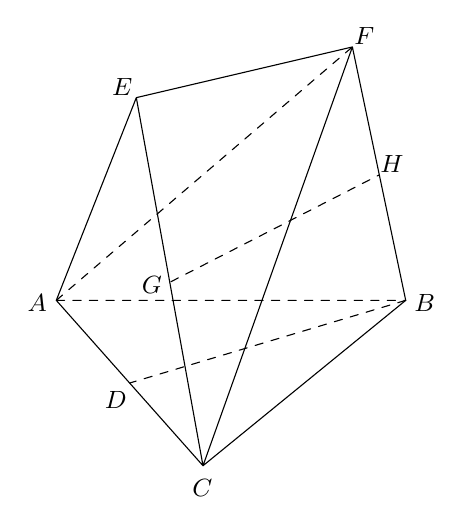
\begin{tikzpicture}[line cap=round,line join=round,font=\small,x=0.03515cm,y=0.03515cm]
% ===== 虚线先画（隐藏棱与辅助线）=====
\draw[dash pattern=on 2.99pt off 2.99pt]
  (0,0)--(106.96,91.54)          % A-F（隐藏棱）
  (0,0)--(126.23,0)              % A-B（隐藏棱）
  (126.23,0)--(26.50,-29.87)     % B-D（辅助线）
  (41.43,6.74)--(116.59,45.29);  % G-H（辅助线，照源实测端点）
% ===== 实线 =====
\draw
  (0,0)--(28.91,73.23)           % E-A
  (28.91,73.23)--(106.96,91.54)  % F-E
  (106.96,91.54)--(126.23,0)     % B-F
  (126.23,0)--(53.00,-59.74)     % C-B
  (53.00,-59.74)--(0,0)          % A-C
  (53.00,-59.74)--(28.91,73.23)  % C-E
  (53.00,-59.74)--(106.96,91.54);% C-F
% ===== 标注（照源字形框中心，显式坐标）=====
\node[anchor=center,inner sep=0] at (-6.87,-1.08) {\(A\)};
\node[anchor=center,inner sep=0] at (133.09,-1.08) {\(B\)};
\node[anchor=center,inner sep=0] at (52.74,-67.82) {\(C\)};
\node[anchor=center,inner sep=0] at (23.79,77.11) {\(E\)};
\node[anchor=center,inner sep=0] at (111.30,95.43) {\(F\)};
\node[anchor=center,inner sep=0] at (21.53,-35.89) {\(D\)};
\node[anchor=center,inner sep=0] at (34.58,5.67) {\(G\)};
\node[anchor=center,inner sep=0] at (121.25,49.16) {\(H\)};
\end{tikzpicture}
\end{center}
\nopagebreak[4]
\end{question}
\begin{question}
\gkti{19}已知数列 \(\{a_n\}\) 的前 \(n\) 项和 \(S_n=3n^2+8n\)，\(\{b_n\}\) 是等差数列，且 \(a_n=b_n+b_{n+1}\)。

（1） 求数列 \(\{b_n\}\) 的通项公式；

（2） 令 \(c_n=\dfrac{(a_n+1)^{n+1}}{(b_n+2)^n}\)，求数列 \(\{c_n\}\) 的前 \(n\) 项和 \(T_n\)。

\end{question}
\begin{question}
\gkti{20}设函数 \(f(x)=x\ln x-ax^2+(2a-1)x\)，\(a\in\mathbf{R}\)。

（1） 令 \(g(x)=f'(x)\)，求函数 \(g(x)\) 的单调区间；

（2） 已知 \(f(x)\) 在 \(x=1\) 处取得极大值，求实数 \(a\) 的取值范围。

\Needspace{0.4\textheight}
\end{question}
\begin{question}
\gkti{21}已知椭圆 \(C\)：\(\dfrac{x^2}{a^2}+\dfrac{y^2}{b^2}=1\)（\(a>b>0\)）的长轴长为 4，焦距为 \(2\sqrt{2}\)。

（1） 求椭圆 \(C\) 的方程；

（2） 过动点 \(M(0,m)\)（\(m>0\)）的直线交 \(x\) 轴于点 \(N\)，交 \(C\) 于点 \(A\)，\(P\)（\(P\) 在第一象限），且 \(M\) 是线段 \(PN\) 的中点，过点 \(P\) 作 \(x\) 轴的垂线交 \(C\) 于另一点 \(Q\)，延长线 \(QM\) 交 \(C\) 于点 \(B\)。

　　① 设直线 \(PM\)、\(QM\) 的斜率分别为 \(k\)、\(k'\)，证明 \(\dfrac{k'}{k}\) 为定值；

　　② 求直线 \(AB\) 的斜率的最小值。
\nopagebreak[4]
\begin{center}% 第 21 题坐标图：按固定源 PDF 矢量路径换算（1 pt → 0.03515 cm）。
% 原点即两轴交点 O（源页 (1052.55, 260.43) pt），y 向上。椭圆半轴 70.84/50.09（比值 √2/2，与题设
% a=2、b=√2 同比例，按比例作图），线宽 0.8pt（源为其余图元 2 倍）；x 轴 −88.55..88.55、y 轴 ±70.84。
% 割线过 A、N、M、P 并向两端延伸（左越 A 15.6pt、右越 P 28.3pt）；竖直线 P–Q 垂直 x 轴；
% 弦 Q–B、A–B。M 为 PN 中点（源图自洽：M 在 y 轴上且为 PN 中点）。图上无实心圆点、坐标轴无刻度。
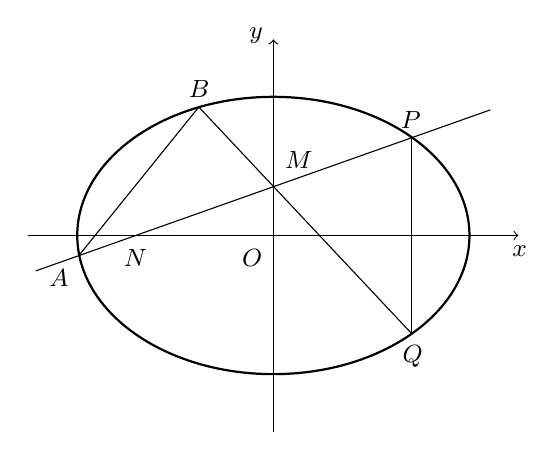
\begin{tikzpicture}[line cap=round,line join=round,font=\small,x=0.03515cm,y=0.03515cm]
% 坐标轴
\draw[->] (-88.55,0)--(88.55,0);
\draw[->] (0,-70.84)--(0,70.84);
% 椭圆（线宽 0.8，与源一致）
\draw[line width=0.8pt] (0,0) ellipse (70.84 and 50.09);
% 割线、竖直线 P–Q、弦 Q–B、弦 A–B
\draw (-85.71,-12.75)--(78.28,45.34);
\draw (49.94,35.42)--(49.94,-35.42);
\draw (49.94,-35.42)--(-26.92,46.40);
\draw (-70.13,-7.09)--(-26.92,46.40);
% ===== 标注（显式坐标，照源字形框中心）=====
\node[anchor=center,inner sep=0] at (-6.26,72.26) {\(y\)};
\node[anchor=center,inner sep=0] at (89.0,-5.59) {\(x\)};
\node[anchor=center,inner sep=0] at (-26.80,52.75) {\(B\)};
\node[anchor=center,inner sep=0] at (49.63,41.76) {\(P\)};
\node[anchor=center,inner sep=0] at (9.19,27.39) {\(M\)};
\node[anchor=center,inner sep=0] at (-49.78,-8.25) {\(N\)};
\node[anchor=center,inner sep=0] at (-7.60,-8.25) {\(O\)};
\node[anchor=center,inner sep=0] at (-77.40,-15.34) {\(A\)};
\node[anchor=center,inner sep=0] at (50.36,-43.68) {\(Q\)};
\end{tikzpicture}
\end{center}
\nopagebreak[4]

\end{question}